% !TEX root = ../thesis.tex

\chapter{Strojové učenie}

\section{Formy strojového učenia a typy dát}
Strojové učnie možeme rozdeliť na tri časti: učenie s učiteľom, učenie bez učiteľa a učenie posilňovaním.

Učenie s učiteľom je forma strojového učenia, pri ktorom majú naše dáta aj určené do ktorej triedy, ktorú chceme predikovať patria. Naše namerané X hodnoty najú svoje y.

Učenie bez učiteľa je prípad kedy naše dáta nemajú určenú triedu, ktorú potrebujeme predikovať. Algoritmus musí najsť triedy sám.

V prípade učnia s posilňovaním je učenie vykonávané formou spätnej väzby, kde v prípade správnej predikcie je algoritmus odmenený a v prípade nesprávnej potrestaný. 

Pre každú formu strojového učenia potrebujeme nejaké dáta, na ktorých sa bude náš model učiť a testovať. Dáta možu byť rôznych formátov ale najčastejšie ide o tabuľy pozostávajúce z uskutočnených meraní - vzoriek. Každá vzorka má svoje atribúty a v prípade učenia s učiteľom aj svoju triedu. 

\subsection{Proces strojového učenia}
Proces strojového učenia pozostáva z viacero časti. Prvou časťou je zber dát. V praxi častokrát dostane Machine learning engineer už pripravené dáta, ak firma zbierala dáta od zákazníkov alebo dostala výsledky prieskumu. Poprípade si vieme dáta zozbierať aj sami, napríklad vytvorením web scrappera, ktorý nám zozbiera dáta z webu.

Ďalšou časťou procesu je predspracovanie dát. Zo zozbieraných dát musíme vybrať dáta ktoré sú pre nás relevantné. Musíme sa usistiť že nemáme nejaké prázdne hodnoty, v takom prípade musíme buď zmazať celé jedno merianie, alebo tam imputovať priemerné hodnoty, Musíme premeniť znakové hodnoty na číselné, pričom musíme zohľadniť rozdiely medzi ordinálnymi a nominálnymi atribútmi. Ak máme veľký nepomer vo veľkosti číselných atribúov, musíme aplikovať škálovanie a/alebo normalizáciu. A v neposlednom rade musíme rozdeliť naše dáta na trénovacie a testovacie. Nesmie nastať situácia aby sme použili časť testovacích dát na trénovanie a naopak.

Keď máme spravené predspracovanie dát, môžeme sa pustiť do výberu modelu. Je ideálne si vyskúšať viacero možných algoritmov a zároveň aj parametrov. Pomocou cross-validácie zitíme ktorý model a jeho nastavenia budú najviac vyhovovať nášmu riešeniu. 

Keď máme náš model natrénvaný, môžeme pristúpiť k ďalšiemu kroku, čo je evaluácia modelu. Necháme zbehnuť náš model na testovacích dátach a necháme ho predikovať hodnoty. 

Ako posledná časť procesu je nasadenie modelu (deploy) do aplikácie. Táto časť procesu nie je súčasťou zadania, avšak ak by sme robili model do praxe, tak by sme napríklad chceli náš model na predikciu kníh, ktoré by sa mohli zákazníkovi páčiť, nasadiť do aplikácie knihkupectva.

\begin{figure}[!ht]
  \centering
  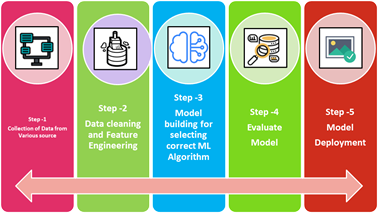
\includegraphics[width=1\textwidth]{figures/process.png}
  \caption{Proces strojové učenia}
  \cite{process}
\end{figure}

\subsection{sickitLarn}


\section{Porovnania cien nehnutelnosti}

\subsection{Lineárna regresia}
